\label{sec:workflow}
% api and sequence

\begin{figure}
    \centering
    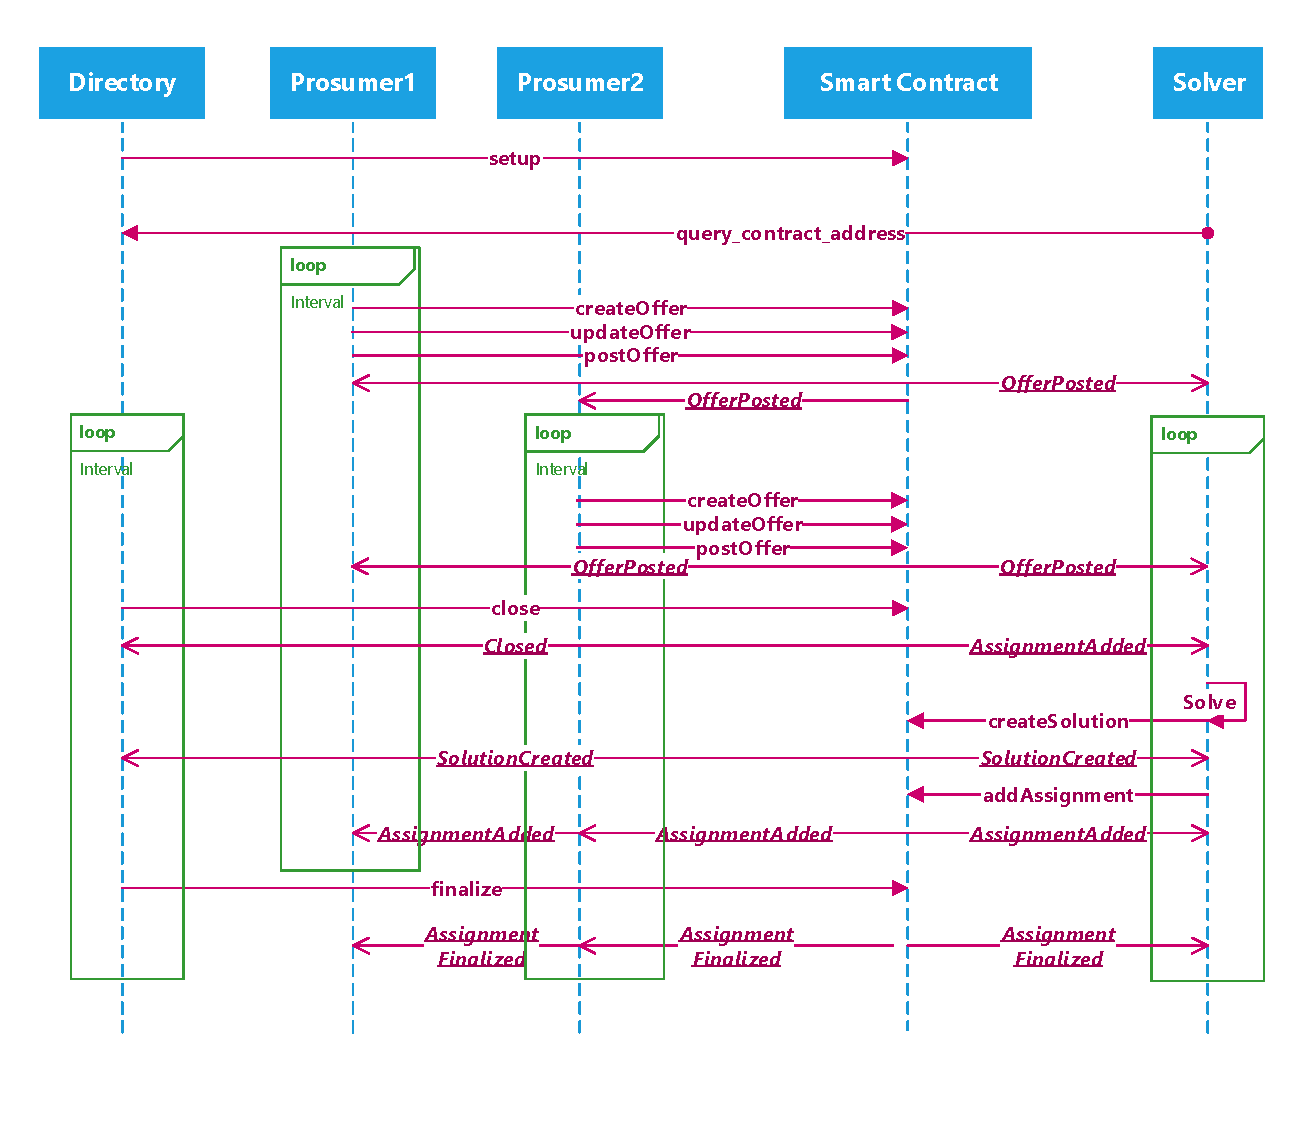
\includegraphics[width=\columnwidth]{Workflow.pdf}
    \caption{Sequence of operations in the transaction management platform.} % Prosumers and Solvers use the directory to find one of the miner nodes running the smart contract. They then connect to the  mining node.}
    \label{fig:workflow}
\end{figure}


\Aron{The figure has not much to do with the current platform. Key functions are missing, and non-existing functions are shown. Needs to be remove or updated!}
\Aron{What is the point of this subsection? This needs to be made clear at the beginning.}
Figure \ref{fig:workflow} describes the workflow of activity in this transaction management platform.  The specific operations in this workflow are described below. Note that the events in this workflow can arrive out of order at the smart contract. %For example, a consumer can request a resource from a time interval that has already been finalized by the smart contract. However, those consumption offers will be rejected.

\begin{itemize}[leftmargin=*]
\setlength{\itemsep}{0pt}%
    \setlength{\topsep}{0pt} 
    \setlength{\partopsep}{0pt}
    \setlength{\parsep}{0pt}
    \setlength{\parskip}{0pt}%
\item Deploying the contract \texttt{(bytecode)}\Aron{Writing ``deployContract'' in the figure suggests that there is a function named ``deployContract'' in the smart contract or the blockchain, which is not true.}: 
Blockchain transaction submitted by a directory actor. \Aron{Directory has not been mentioned in the text before!} The transaction deploys the smart contract, making it available for all participants to use. The blockchain returns the address of the deployed contract.\Aron{This is kind of obvious.}
\item \texttt{Connect}: \Aron{This is practically just establishing a TCP connection. Why do we mention this?!} Any new participant first connects to the directory. The directory can run an optional mixing service\Aron{Anonymization needs to be discussed more detail or omitted.}, providing the participants with an anonymous identifier.
\item \texttt{query\_contract\_address}:  This is an off-blockchain communication between participants and the directory, which returns the address of the smart contract. 
\item \texttt{registerProsumer(uint64 prosumer)}: \Aron{Remove this! It was not listed in the contract (see FSolidM section), and it has not been implemented.} Each prosumer registers with the smart contract, providing an anonymous identifier.
\item \texttt{ProsumerRegistered}: \Aron{Again, what is this doing here? There is nothing like this in the platform.} Event broadcast by the smart contract, notifying prosumers that they have registered. 
\item \texttt{postOffer(assetID, price)}: \Aron{Fuction signatures are all wrong...} smart contract function called by a prosumer, publicly posting an offer to produce or consume a resource. The resource type is encoded in the assetID and checked by the smart contract.
\item \texttt{OfferPosted(offerID, assetID, price)}: event broadcast by the smart contract, notifying solvers that an offer was posted.
%\item \texttt{Solve} : Once offers have been posted the Solver begins solving for potential matchings of the offers of which it has been notified. \Aron{This is not an interaction, so it should not be on this list. Further, we don't assume anything about solvers, so we really shouldn't discuss their internal working here.}
\item \texttt{createSolution(uint64 solverID)}: The Solver sends a request to the smart contract to tell it that a new solution has been found..
\item \texttt{SolutionCreated}: event broadcast by the smart contract, notifying the solver that it can submit the trades that constitute the new solution.
\item \texttt{addAssignment(uint64 solutionID, uint64 sellerID, uint64 buyerID, uint64 time, uint64 power)}: smart contract function called by the solver, which posts the trades to the solution created previously on the blockchain. As the trades are added the smart contract verifies that each is a valid trade and does not violate any of the system constraints.
\item \texttt{AssignmentAdded}: An event broadcast by the smart contract notifying the solver and the prosumers that a trade has been added to a potential solution. 
\item \texttt{finalize} : smart contract function called by the directory causing the contract to stop accepting new solutions which include the interval being finalized. The contract selects the best solution\footnote{The smart contract keeps track of the best solution as a new solution is added. This ensures that it does not have to search the list of solutions to select the best solution (max objective value) during finalization.} and broadcasts the \texttt{Finalize} event. 
\item \texttt{Finalized} : event broadcast by the smart contract notifying the solver to begin working on the next interval
\item \texttt{AssignmentFinalized}: An event broadcast by the smart contract notifying participants off all trades that were in the final accepted solution. 
\end{itemize}
\Aron{This subsection needs to be rewritten almost completely!}